Ce chapitre résume le travail de comparaison de la loi incompressible \cacro{PP98} et de deux cas de la loi compressible isentrope-polytrope. Dans le premier cas, elle est fermée tel que $\gamma = 1$ (isotherme) et dans le second, tel que $\gamma = 5/3$ (adiabatique). Cette comparaison est effectuée dans deux jeux de données de compressibilité différente issus de \cacro{PSP} afin de comprendre l'apport de la loi polytrope dans l'estimation du taux de chauffage dans le vent solaire. Ce travail a fait l'objet d'une publication, \cite{simon_general_2021}, puis a été étendu statistiquement dans le cadre d'une étude préliminaire dans des données relevées dans la magnétogaine terrestre par la mission \cacro{MMS}. La formulation des lois compressibles utilisée est la formulation f1 donnée par la loi exacte générale \eqref{eq:turb_elg_f1}. 

\section{Données et conditions d'application d'une loi exacte dans des observations issues d'une seule sonde}
\label{sec-141}

Le 12 août 2018, \cacro{PSP} commence son voyage à bord d'une fusée Delta IV-Heavy. Cette mission lancée par la \sacro{NASA} devra s'approcher au maximum du Soleil afin de permettre la compréhension de la dynamique insufflée par le Soleil dans son environnement, du chauffage et de l'accélération de la couronne solaire et du vent solaire à ceux des particules énergétiques [\cite{fox_solar_2016}]. Un tel objectif résonne avec l'application des lois exactes dans les données afin d'estimer le taux de chauffage turbulent [\cite{parashar_observations_2022}]. De plus, comme indiqué sur la \figref{fig:schema_thermo}, le $\gamma$ estimé près du Soleil est plus proche, voire supérieur, de 5/3 que de 1. Relaxer l'isothermie dans la loi exacte et y regarder une loi polytrope y semble donc plus réaliste. 

Pour estimer le taux de chauffage avec une loi exacte \cacro{MHD}, nous avons besoin du champ magnétique et des moments mono-fluides de la fonction de distribution. Ces données sont relevées par deux expériences de \cacro{PSP} (voir la \figref{fig:sonde_PSP}) : \cacro{FIELDS} et \cacro{SWEAP}. 
\begin{figure}[!ht]
 \centering
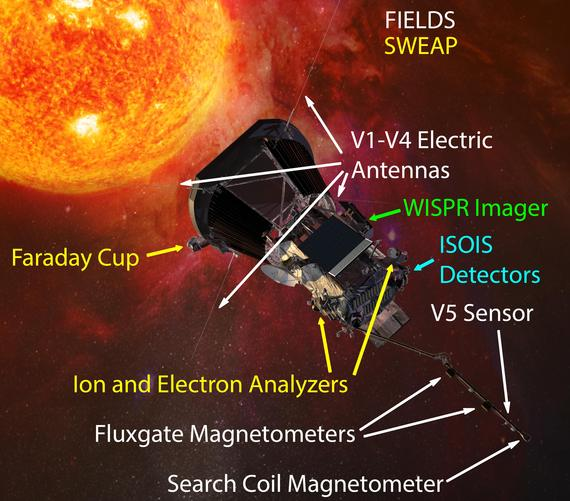
\includegraphics[width=0.9\linewidth,trim=0cm 0cm 0cm 0cm, clip=false]{./Mainmatter/Part_1/images/PSP_All_Instruments}
\cprotect\caption{Localisation des instruments de mesure sur \cacro{PSP}. Les instruments de l'expérience \cacro{FIELDS} sont notés en blanc, et ceux de \cacro{SWEAP} en jaune. Les données utilisées ici proviennent des magnétomètres à saturation (Fluxgate Magnetometers, \cacro{MAGs}) situés sur le bras et de la coupe de Faraday (Faraday Cup, \cacro{SPC}) située juste à côté du bouclier et orientée vers le Soleil. Crédits : la page web de \cacro{FIELDS} (\verb|fields.ssl.berkeley.edu|) et Johns Hopkins University Applied Physics Laboratory.}
\label{fig:sonde_PSP}
\end{figure}
 
 \cacro{FIELDS} [\cite{bale_fields_2016}] mesure le champ magnétique grâce à deux magnétomètres à saturation (\og fluxgate \fg{} en anglais), \cacro{MAGs}, mesurant la composante continue (DC) et les fluctuations à basse fréquence (MHD-ionique) du champ,  et un de type fluxmètre (\og search-coil \fg{}), \cacro{SCM}, donnant accès aux hautes fréquences (ionique-électronique). \cacro{SWEAP} [\cite{kasper_solar_2016}] est quant à elle composée d'une coupe de Faraday (\og Faraday Cup \fg{}), \cacro{SPC}, mesurant les flux globaux ionique et électronique, et d'analyseurs électrostatiques d'ions et d'électrons, \cacro{SPAN}, permettant de séparer leur état de charge. Notre étude concernant plutôt les échelles MHD, les données utilisées proviennent des instruments \cacro{MAGs} et \cacro{SPC}. 

Les données publiquement disponibles au moment où cette étude a été menée (fin 2020) provenaient des quatre premières orbites (\figref{fig:orbit_PSP}). 
\begin{figure}[!ht]
 \centering
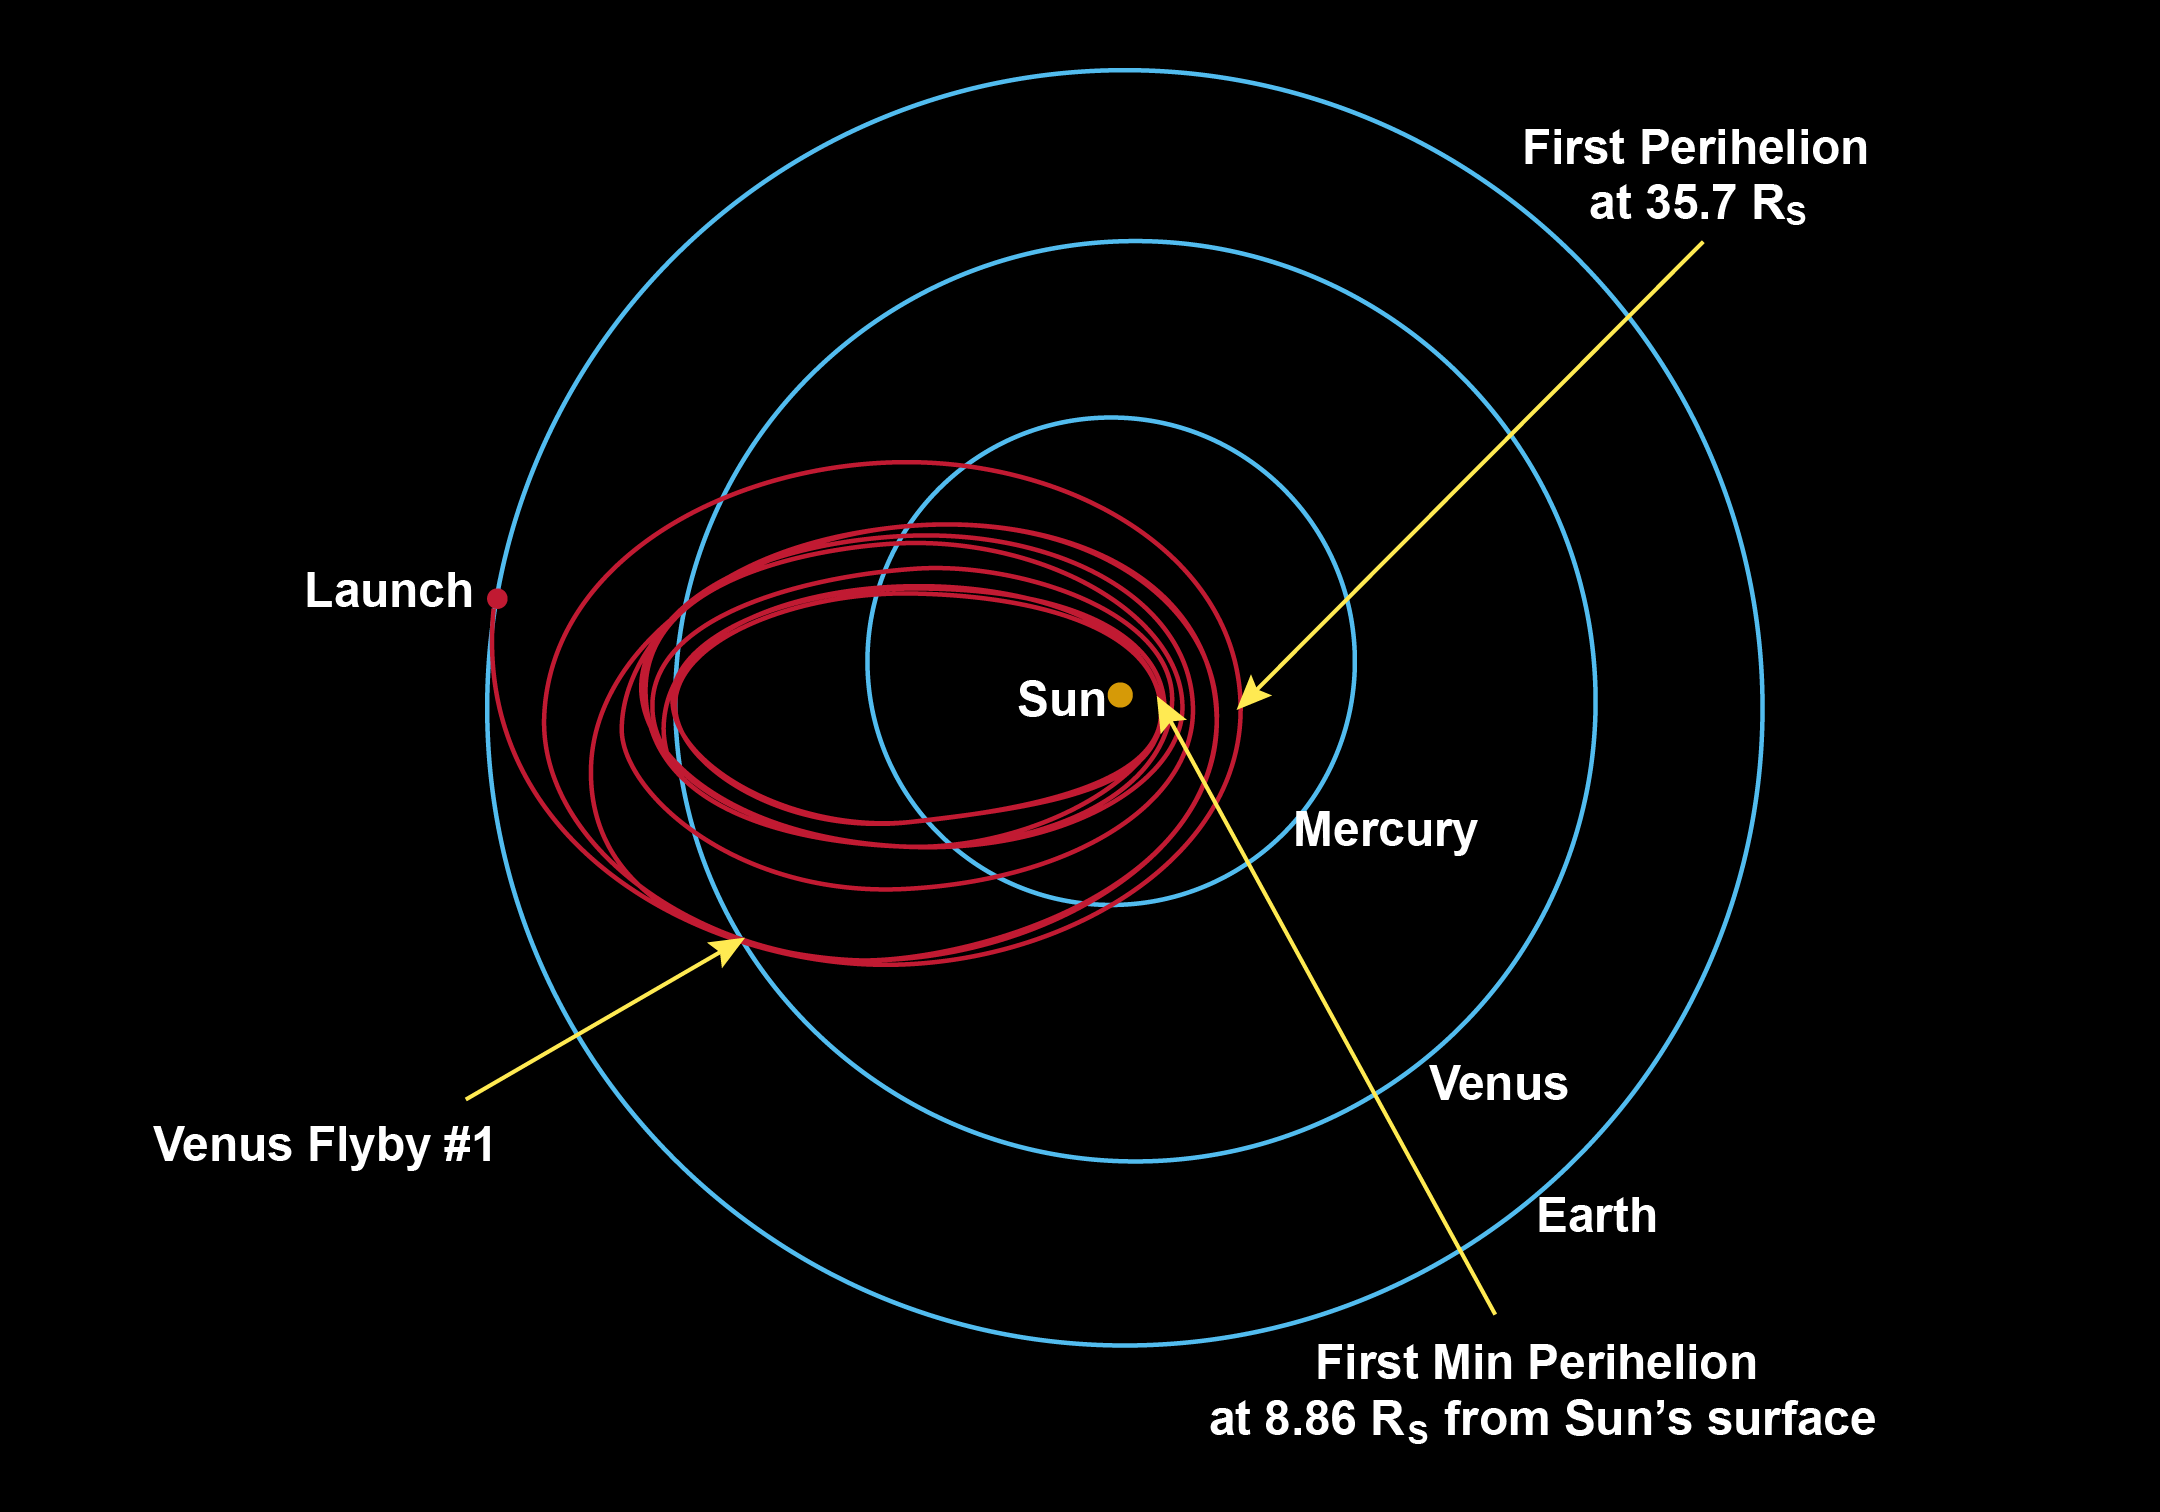
\includegraphics[width=0.9\linewidth,trim=0cm 0cm 0cm 0cm, clip=false]{./Mainmatter/Part_1/images/16-00815_MissionDesign}
\cprotect\caption{Orbites de \cacro{PSP} depuis la date de lancement, le 12 août 2018 à 7h31 \cacro{UTC}. Le premier périhélie à $\SI{35.7}{Rs}$ a été atteint le 6 novembre 2018 à 03h27 \cacro{UTC}. Crédits : la page web de \cacro{PSP} (\verb|http://parkersolarprobe.jhuapl.edu|) et Johns Hopkins University Applied Physics Laboratory.}
\label{fig:orbit_PSP}
\end{figure}
Nous avons choisi d'analyser les données relevées lorsque \cacro{PSP} était proche de son premier périhélie atteint le 6 novembre 2018 à 03h27 \cacro{UTC} vers $\SI{35.7}{Rs}$. Autour de cette position, les données sont relevées dans le vent solaire près du Soleil. Mais peu de lots de données comprenant conjointement les relevés provenant de \cacro{SPC} et ceux provenant de \cacro{MAGs} étaient assez complets pour être traités. Finalement, le jeu choisi a été relevé le 4 novembre entre 00h00 et 02h30. Les données provenant de \cacro{MAGs} y sont résolues à une cadence d'environ $\SI{7}{ms}$ sans temps manquant tandis que celles provenant de \cacro{SPC} sont résolues à $\SI{0,873}{s}$ et montrent $0.15\%$ de temps manquants situés entre 01h08 et 01h13. Ces trous seront comblés par interpolation linéaire et, afin d'avoir la même cadence, les données \cacro{MAGs} sont rééchantillonnées sur la cadence de \cacro{SPC}. Les données analysées sont montrées sur la \figref{fig:data_PSP}.  
 \begin{figure}[!ht]
 \centering
 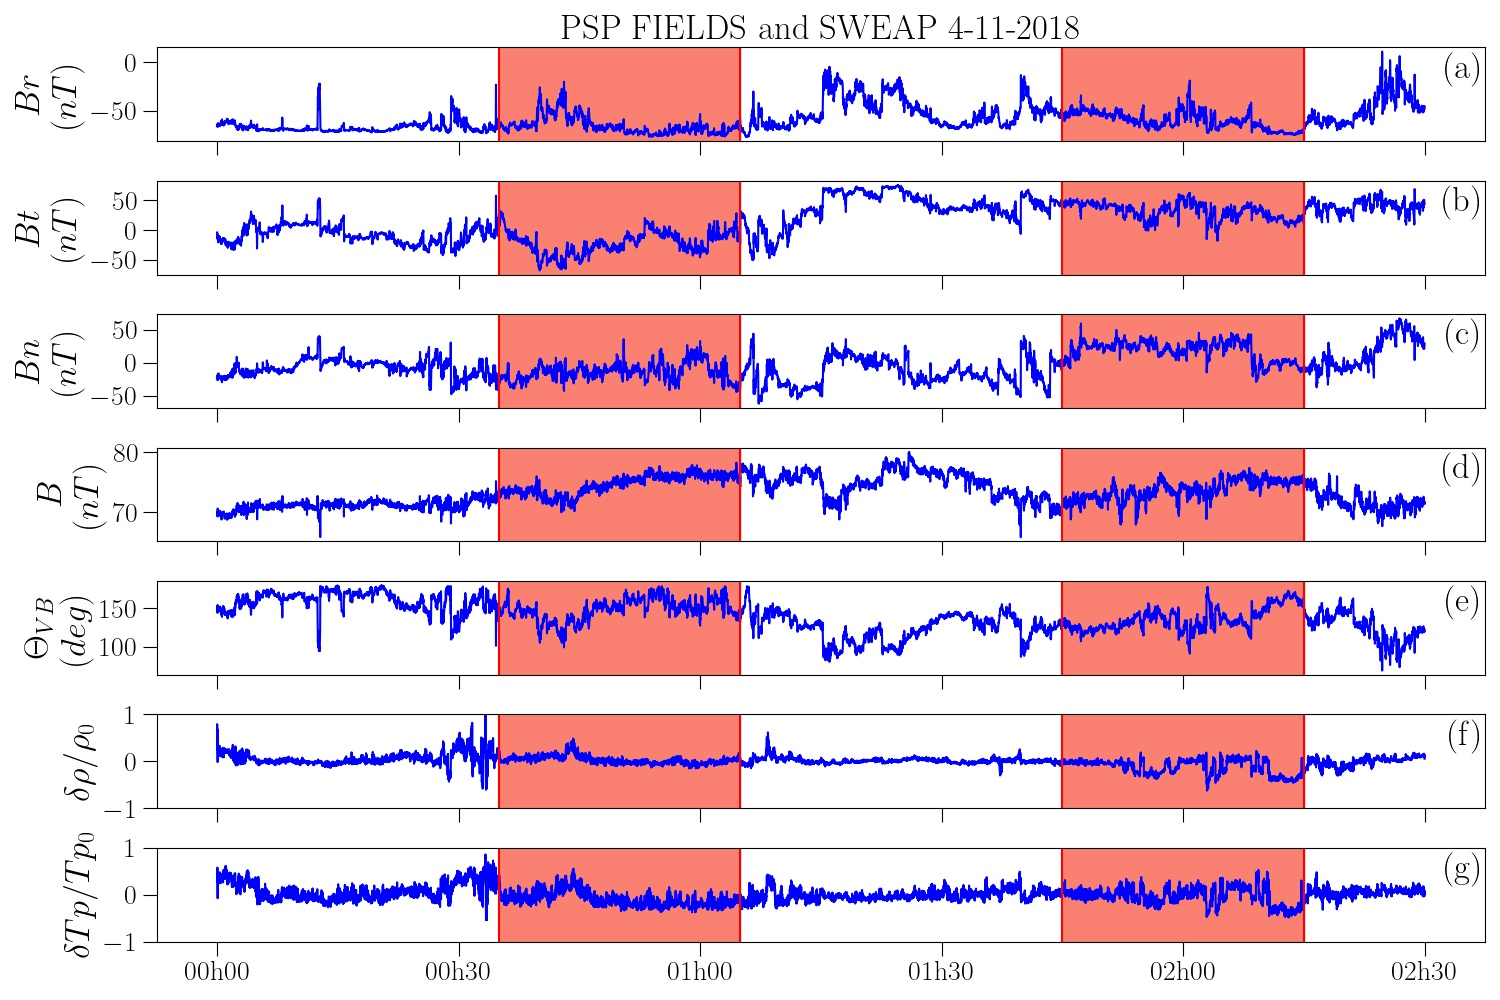
\includegraphics[width=\linewidth,trim=0cm 0cm 0cm 0cm, clip=false]{./Mainmatter/Part_1/images/Fig_04112018H_00_panel}
 \cprotect\caption{Données \cacro{PSP} mesurées dans l'héliosphère interne le 4 novembre 2018. (a) à (c) : les trois composantes du champ magnétique dans le système de représentation \cacro{RTN}. (d) : Norme du champ magnétique. (e) : angle entre le champ de vitesse du fluide et le champ magnétique. (f) et (g) : fluctuations de densité et température relative des protons. Les zones rouges représentent les sous-intervalles utilisés pour le calcul des taux de cascade.}
 \label{fig:data_PSP}
 \end{figure}

Les sous-intervalles choisis pour le calcul des taux de cascade sont marqués en rouge et sont associés à deux niveaux de compressibilité différents. La compressibilité noté $c$ est calculée en prenant l'écart-type, $\text{std}$, des fluctuations de densité, c'est-à-dire $c = \text{std}(\frac{\rho - \rho_0}{\rho_0}) = \text{std}(\frac{\delta \rho}{\rho_0})$. Le premier sous-intervalle, de 00h35 à 01h05 a une compressibilité très faible, $c \sim 8\%$, tandis que le second, de 01h45 à 02h15, est plus compressible, $c \sim 20\%$. Grâce à ces deux intervalles, nous pouvons étudier l'impact des différents niveaux de fluctuations de densité sur le taux de cascade calculé avec la loi isentrope-polytrope et la loi incompressible.

Ces choix de sous-intervalles ont été effectués en considérant un certain nombre d'hypothèses permettant de calculer un taux de cascade tout en réduisant l'incertitude du résultat. Les séries étant temporelles, on utilise l'hypothèse de Taylor\footnote{La validité de l'hypothèse de Taylor dans le vent solaire et en particulier le long de la trajectoire de \cacro{PSP} peut être remise en question [\cite{treumann_applicability_2019,chhiber_contextual_2019}] mais l'obtention d'une hypothèse de remplacement est encore une question ouverte [\cite{parashar_observations_2022}].} [\cite{taylor_spectrum_1937}] qui présuppose que les variations temporelles relevées par la sonde peuvent être interprétées comme des variations spatiales convectées par le flot de plasma à la vitesse moyenne $\boldsymbol{v_0}$. Ainsi, on peut estimer l'incrément spatial $\boldsymbol{\ell}$ à partir de l'incrément temporel $\tau $ via $ \boldsymbol{\ell} \sim \boldsymbol{v_0} \tau$. L'utilisation de l'hypothèse de Taylor donne donc accès aux échelles spatiales dans la direction moyenne du flot. Or le couplage entre le champ magnétique et le fluide implique une forte anisotropie entre les directions parallèle et perpendiculaires au champ magnétique. Par conséquent, si l'angle entre la vitesse et le champ magnétique, $\theta_{VB}$, varie trop fortement, d'importantes variations pourront apparaître dans les résultats du taux de cascade, comme l'ont observé [\cite{hadid_energy_2017}]. Les intervalles ont donc été choisis tel que $\theta_{VB}$ soit relativement stationnaire (ligne (e) de la \figref{fig:data_PSP}). On a aussi considéré des séries temporelles relativement stationnaires pour les autres quantités afin d'assurer une certaine stationnarité/homogénéité statistique. 

L'estimation des moyennes dans le calcul du taux de cascade demande une statistique suffisante, c'est-à-dire des intervalles de durée supérieure à plusieurs fois le temps de corrélation des fluctuations turbulentes [\cite{coburn_third-moment_2015}]. 
[\cite{parashar_measures_2020}] ont estimé le temps de corrélation des données relevées par \cacro{PSP} entre le 3 et le 10 novembre avec des intervalles glissants de 4h, 8h et 24h. En se fiant à cette estimation, le temps de corrélation pour les données utilisées ici (le 4 novembre entre 00h00 et 02h30) est autour de $\SI{500}{s}$, c'est-à-dire un peu moins du tiers de la longueur de nos sous-intervalles ($\SI{30}{min}$). On supposera donc que leur durée convient au calcul d'un taux de cascade. 

\begin{figure}[!ht]
 \centering
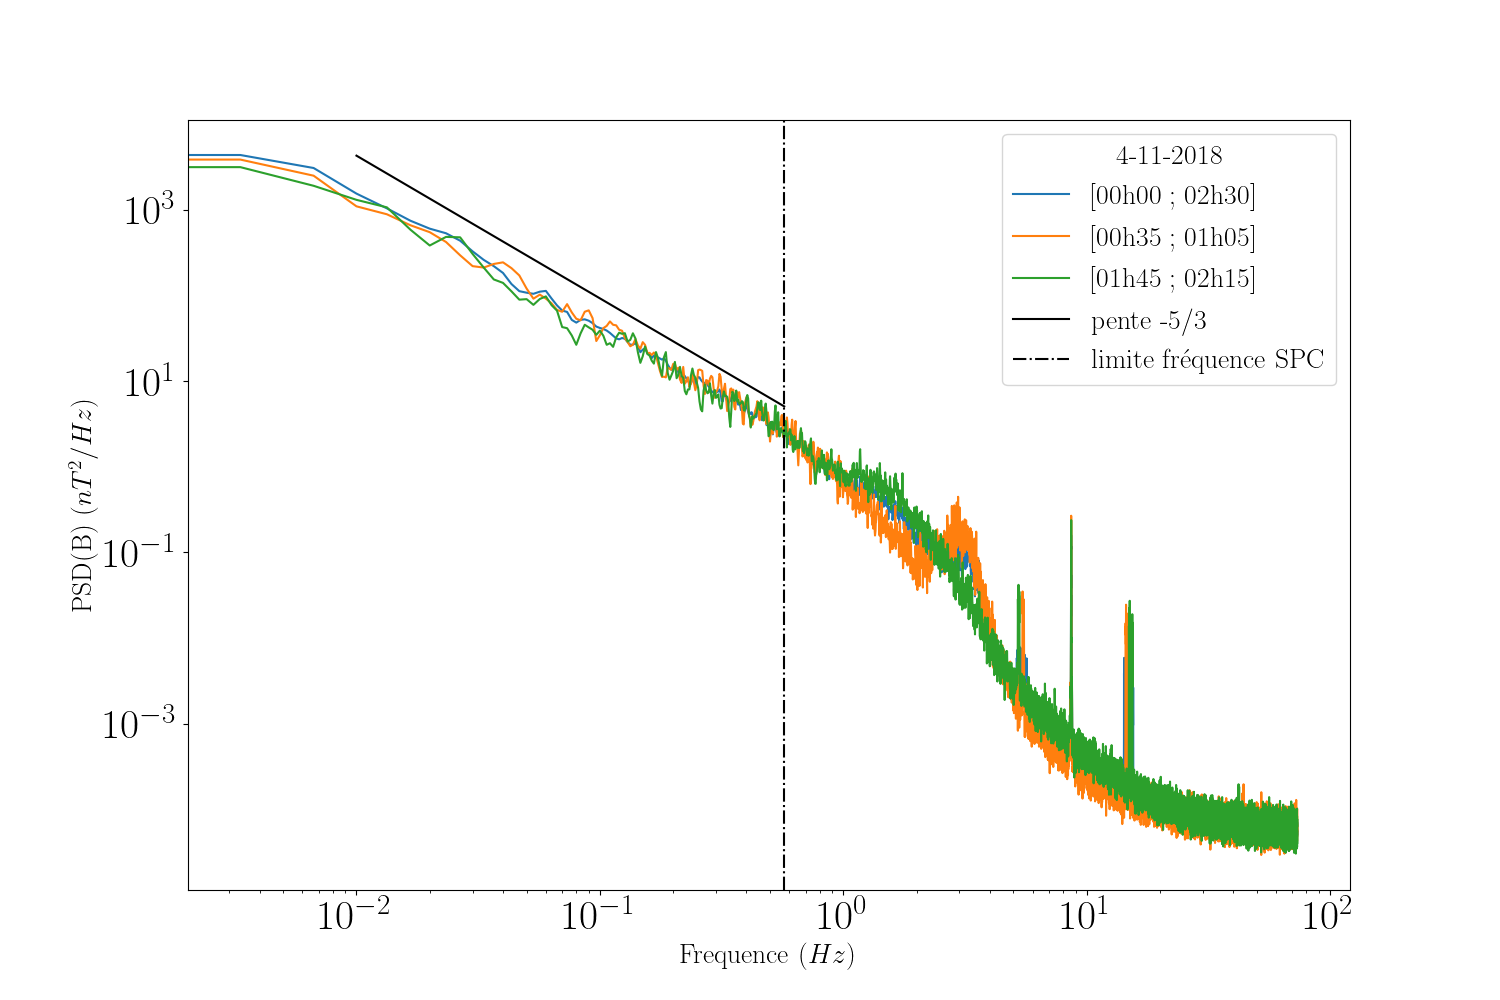
\includegraphics[width=\linewidth,trim=0cm 0cm 0cm 0cm, clip=false]{./Mainmatter/Part_1/images/Fourier2}
\cprotect\caption{Spectre des fluctuations magnétiques pour l'intervalle complet de données (bleu), et les sous-intervalles (orange et vert) obtenue avec les données \cacro{MAGs} non rééchantillonnées à la cadence de \cacro{SPC}. La ligne noire continue indique la pente attendue dans la zone MHD (spectre de type Kolmogorov en $-5/3$) et l'axe vertical la fréquence maximale accessible avec la cadence de \cacro{SPC}.}
\label{fig:spec_PSP}
\end{figure}

Sur la \figref{fig:spec_PSP}, sont tracés les spectres des fluctuations magnétiques obtenus avec les données \cacro{MAGs} non rééchantillonnées de l'intervalle complet et des deux sous-intervalles. Les fréquences qui nous intéressent sont les fréquences inférieures à la cadence de \cacro{SPC}. Pour ces fréquences, la pente des spectres est proche de $-5/3$ (attendue dans la zone \cacro{MHD}). La loi exacte du modèle \cacro{MHD} dérivée dans le Chapitre \ref{ch-13} y semble donc applicable. 
 
 \section{Comparaison des lois incompressible et compressible-isentrope-polytrope avec \ensuremath{\gamma = 1} (isotherme) et \ensuremath{\gamma = 5/3} (adiabatique)}
 \label{sec-142}

Pour ce qui est de la forme de la loi exacte, l'utilisation d'une seule sonde impose deux autres hypothèses. La première correspond à la négligence des termes sources. En effte, ces derniers ne peuvent pas être calculés à cause de leur dépendance en des dérivées locales ($\nabla$ et $\nabla'$) qui ne peuvent être estimées qu'avec des missions multi-sondes telles que \cacro{MMS} ou \cacro{CLUSTER} en orbite autour de la Terre [\cite{andres_energy_2019}]. Physiquement, une telle hypothèse pourrait avoir un impact significatif. Mais d'après l'étude numérique de [\cite{andres_energy_2019}] en turbulence MHD subsonique sur une loi exacte isentrope-isotherme formulée similairement à \eqref{eq:turb_elg_f1} (formulation qui sera considérée ici), les termes flux donnés ci-dessous \eqref{eq:obs_F1} sont dominants tandis que les autres termes sont négligeables ou se compensent. La deuxième hypothèse est celle d'isotropie des fluctuations qui permet d'intégrer tridimensionnellement la loi exacte dans une boule de rayon $\ell = |\boldsymbol{\ell}|$. Cette hypothèse simplificatrice est largement utilisée [\cite{parashar_observations_2022}] mais sa validité peut être remise en cause par l'anisotropie du plasma due au champ magnétique\footnote{Un taux de cascade incompressible intégré axisymétriquement a été investigué par \cite{andres_incompressible_2022} mais une extension compressible reste à faire.}. L'expression du taux de cascade calculée ici est alors : 
\begin{equation}
\label{eq:obs}\varepsilon = F_1 + F_2,
\end{equation}
avec
\begin{eqnarray}
\label{eq:obs_F1} F_1 &=& -\frac{3}{4|\boldsymbol{v_0}|\tau}\left<(\delta (\rho\boldsymbol{v}) \cdot \delta \boldsymbol{v}+ \delta (\rho\boldsymbol{v_A}) \cdot \delta \boldsymbol{v_A}) \delta \boldsymbol{v}  -(\delta (\rho\boldsymbol{v_A}) \cdot \delta \boldsymbol{v}  + \delta (\rho\boldsymbol{v}) \cdot \delta \boldsymbol{v_A}  ) \delta \boldsymbol{v_A} \right> \nonumber, \\ &&\\
\label{eq:obs_F2} F_2 &=& -\frac{3}{4|\boldsymbol{v_0}|\tau}\left<2 \delta \rho  \delta u  \delta \boldsymbol{v}\right>.
\end{eqnarray}
$F_1$ est la contribution dite Yaglom compressible, ne s'annulant pas dans la limite incompressible, tandis que $F_2$ est la contribution d'énergie interne, dépendant des fermetures compressibles. $\rho$ et $u$ y sont calculés pour des cas particuliers de la fermeture isentrope-polytrope définies dans la \tabref{tab:fermetures} :
\begin{itemize}
    \item incompressible (IMHD) : $\rho = \rho_0$, pas de $u$ nécessaire (cette fermeture permet de retrouver la loi \cacro{PP98}),
    \item isentrope-isotherme (CMHDi): $u = c_s^2 \ln(\frac{\rho}{\rho_0})$ obtenu avec la fermeture isentrope-polytrope et $\gamma = 1$,
    \item isentrope-adiabatique (CMHDp) : $u = \frac{c_s^2 -c_{s0}^2}{\gamma(\gamma -1)}$ obtenu avec la fermeture isentrope-polytrope et $\gamma = 5/3$.
\end{itemize}
La vitesse du son $c_s$ est obtenue grâce à la relation des gaz parfaits $c_s^2 = \gamma k_B T_p /m_p$, avec $k_B$ la constante de Boltzmann, $m_p$ la masse des protons, et $T_p$ la température locale des protons. $c_{s0}$ provient de la relation des gaz parfaits calculée avec la température moyenne des protons.
\begin{figure}[!ht]
 \centering
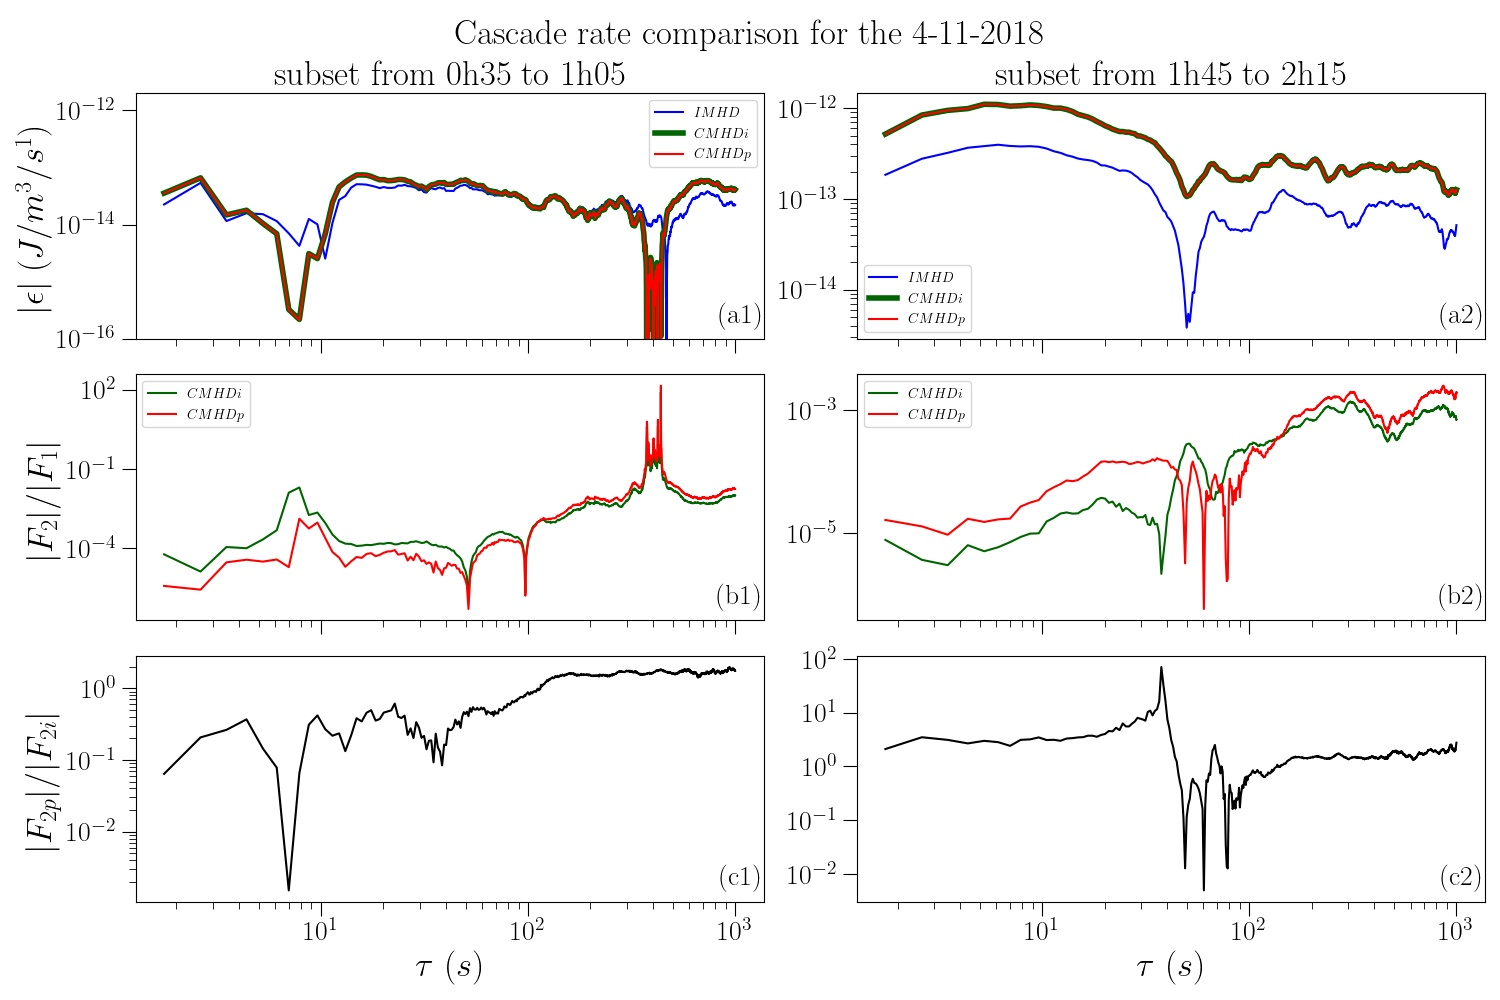
\includegraphics[width=\linewidth,trim=0cm 0cm 0cm 0cm, clip=false]{./Mainmatter/Part_1/images/Fig_04112018H_00_results}
\caption{Comparaison des taux de cascade obtenus avec l'expression de la loi exacte \eqref{eq:obs} et les différentes fermetures pour les sous-intervalles $\{$00h35–01h05$\}$ (à gauche) et $\{$01h45–02h15$\}$ (à droite). (a1)–(a2) : valeur absolue des taux de cascade obtenus avec les fermetures incompressible (IMHD) en bleu, compressibles isentrope-isotherme (CMHDi) en vert et adiabatique (CMHDp) en rouge. (b1)–(b2) : ratio entre la contribution d'énergie interne $F_2$ \eqref{eq:obs_F2} et celle Yaglom compressible $F_1$ \eqref{eq:obs_F1} dans le cas isotherme (vert) et le cas adiabatique (rouge). (c1)–(c2) : ratio entre les contributions de l'énergie interne adiabatique $F_{2p}$ et isotherme $F_{2i}$.}
\label{fig:loi_PSP}
\end{figure}

Sur la \figref{fig:loi_PSP} apparaissent les résultats pour les deux sous-intervalles, le quasi-incompressible à gauche (1) et le plus compressible à droite (2). La première ligne ((a1) et (a2)) montre l'estimation du taux de cascade avec la fermeture IMHD en bleu, la loi CMHDi en vert et CMHDp en rouge. Sur la deuxième ligne ((b1) et (b2)), la contribution d'énergie interne $F_2$ est comparée à la contribution $F_1$ dans les cas isotherme (vert) et adiabatique (rouge). L'impact de la fermeture thermodynamique n'étant portée que par $F_2$, le ratio entre les $F_2$ adiabatique ($F_{2p}$) et isotherme ($F_{2i}$) est donné sur la troisième ligne ((c1) et (c2)).

N'est représentée que la valeur absolue des différentes quantités puisque leur signe nécessite des intervalles plus longs pour statistiquement converger [\cite{coburn_third-moment_2015}, \cite{hadid_energy_2017}]. La question de l'inversion de la cascade potentiellement visualisée à travers le signe du taux ne peut donc pas être étudiée ici. Un taux $\varepsilon$ en valeur absolue quasi-constant peut par contre témoigner d'une convergence. On va donc utiliser la quasi-constance de $\varepsilon$ pour définir une zone inertielle. Pour le premier intervalle, sur le graphique (a1) de la \figref{fig:loi_PSP}, les $\varepsilon$ montrent des variations avant $\tau \sim \SI{10}{s}$ et après  $\tau \sim \SI{400}{s}$ et restent quasiment constant au centre. On supposera donc que cette zone centrale correspond à une zone inertielle. À grande échelle, ces variations proviennent de $F_1$ et se reflètent dans la brusque augmentation apparaissant sur le graphique (b1) de la \figref{fig:loi_PSP}. Ils s'avère que ces variations sont accompagnées de changements de signe. Pour le second intervalle, sur le graphique (a2) de la \figref{fig:loi_PSP}, le signe ne varie pas, il reste positif contrairement à ce que pourrait laisser présager le creux apparaissant en $\tau \sim \SI{50}{s}$. En se fiant à la quasi-constance du niveau de $\varepsilon$, nous limitons l'interprétation d'une zone inertielle à l'intervalle $\tau \in [50;800]\SI{}{s}$. 

 Le graphique (a2) de la \figref{fig:loi_PSP} met en avant le rôle de la compression dans le taux de cascade : les taux de cascade compressibles sont plus élevés d'un facteur 2 à 3 par rapport au taux incompressible, alors que le graphique (a1) de la \figref{fig:loi_PSP} provenant de données bien moins compressible montre des niveaux similaires. Cette observation coïncide avec de précédentes, issues de données du vent solaire [\cite{banerjee_scaling_2016}, \cite{hadid_energy_2017}, \cite{andres_evolution_2021}]. Par contre, les deux modèles compressibles montrent les mêmes résultats. La raison de cette convergence est révélée par les graphiques (b1) et (b2) de la \figref{fig:loi_PSP} : la contribution de $F_2$ est bien négligeable devant celle de $F_1$. Le facteur 3 observé précédemment provient donc de la prise en compte de la densité dans $F_1$.  Même si l'impact du terme dépendant de la fermeture à une importance moindre dans le taux total, nous pouvons en examiner l'effet sur les graphiques (c1) et (c2) de la \figref{fig:loi_PSP}. Aux grandes échelles ($\tau > \SI{100}{s}$), les deux fermetures apportent une contribution similaire tandis qu'à plus petite échelle (hors de la suspectée zone inertielle pour le deuxième intervalle), un ordre de grandeur de différence apparaît. Dans le cas du premier intervalle, la fermeture isotherme contribue plus que l'adiabatique tandis que dans le cas du deuxième intervalle, c'est le contraire. Une interprétation complète de cette différence de comportement ne peut être apportée avec cette étude de cas et nécessite une analyse statistique. Cette analyse, effectuée ultérieurement par \cite{brodiano_statistical_2022} dans les données \cacro{PSP} montre que $\left<F_2\right>$ (en notant $\left<\right>$ la moyenne sur les échelles et en adoptant nos notations des contributions aux taux de cascade) apparaît statistiquement un à deux ordres de grandeur en dessous de $\left<F_1\right>$, et que le facteur $\num{3}$ entre les taux compressibles et le taux incompressible n'est pas retrouvé sauf pour des cas particuliers. Les cas que nous avons étudiés semblent donc dans la norme pour le premier point vérifié, mais, pour le dernier point, notre deuxième sous-intervalle entre dans la classe des cas particuliers. Ils montrent aussi que plus la compressibilité est forte, plus $\left<F_2\right>$ peut venir concurrencer $\left<F_1\right>$ voire, pour certains cas, le surpasser. Près du Soleil, ils notent aussi que $\left<F_{2p}\right>$ est supérieur à $\left<F_{2i}\right>$ en moyenne.

Cette étude de cas préliminaire, publiée dans \cite{simon_general_2021} et validée statistiquement par \cite{brodiano_statistical_2022}, a donc permis de visualiser l'impact de la compression sur l'estimation du taux de cascade et l'apport potentiel d'une fermeture par rapport à une autre dans des données réelles du vent solaire. 

\section{Application statistique préliminaire dans des données localisées dans la magnétogaine terrestre}
\label{sec-143}

Le plasma dans la magnétogaine est plus compressible que dans le vent solaire [\cite{hadid_compressible_2018}] et d'après \cite{livadiotis_long-term_2018}, $1<\gamma<5/3$. Il est aussi exploré par de multiples missions, en particulier des missions multi-sondes comme \cacro{MMS} qui comprend quatre satellites en orbite autour de la Terre depuis 2015 (\figref{fig:MMS}). 
\begin{figure}[!ht]
 \centering
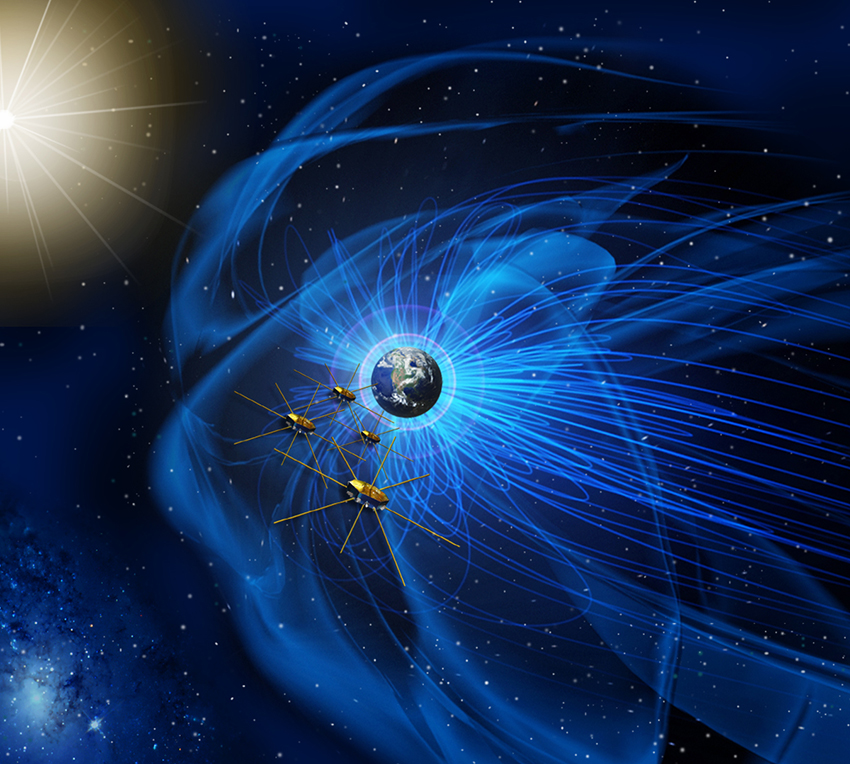
\includegraphics[width=0.7\linewidth,trim=0cm 6cm 6cm 4cm, clip=true]{./Mainmatter/Part_1/images/MMS_mission}
\cprotect\caption{Vue d'artiste de la mission \cacro{MMS}. Crédits : la page web de \cacro{MMS}/\cacro{NASA} (\verb|https://www.nasa.gov/mission_pages/mms|).}
\label{fig:MMS}
\end{figure}

À partir d'une douzaine de cas parmi ceux utilisés par \cite{andres_energy_2019}, nous avons vérifié si l'on retrouve, dans la magnétogaine, les résultats de notre étude de cas effectuée avec les données de \cacro{PSP}. Les données utilisées ont été relevées par les instruments \cacro{FPI} pour ce qui est des moments de la fonction de distribution des particules, et \cacro{FGM}, pour le champ magnétique, pendant 12 intervalles de temps entre 2015 et 2017. L'étude, similaire à celle effectuée avec les données de \cacro{PSP}, est menée séparément sur les quatre satellites de la constellation (48 résultats). 

Concernant les quantités estimées, les notations sont les mêmes que celles utilisées dans la section \ref{sec-133}. La \figref{fig:loi_MMS} montre l'emplacement des 48 résultats pour lesquels les fluctuations de densité (compressibilité $c$) varie de $20\%$ à $60\%$ (visualisé via l'échelle de couleur) dans deux diagrammes ayant pour abscisse le rapport entre les taux moyen compressible $\left<\varepsilon_{CMHDp}\right>$ obtenu avec $\gamma = 5/3$ (loi adiabatique, CMHDp) et incompressible $\left<\varepsilon_{IMHD}\right>$. Le diagramme de gauche a pour ordonnée le rapport entre les contributions d'énergie interne $\left<F_{2p}\right>$ et Yaglom compressible $\left<F_{1}\right>$ de la loi adiabatique et celui de droite le rapport entre les contributions d'énergie interne adiabatique et isentrope-isotherme, respectivement $\left< F_{2p} \right>$ et $\left< F_{2i} \right>$. 
\begin{figure}[!ht]
 \centering
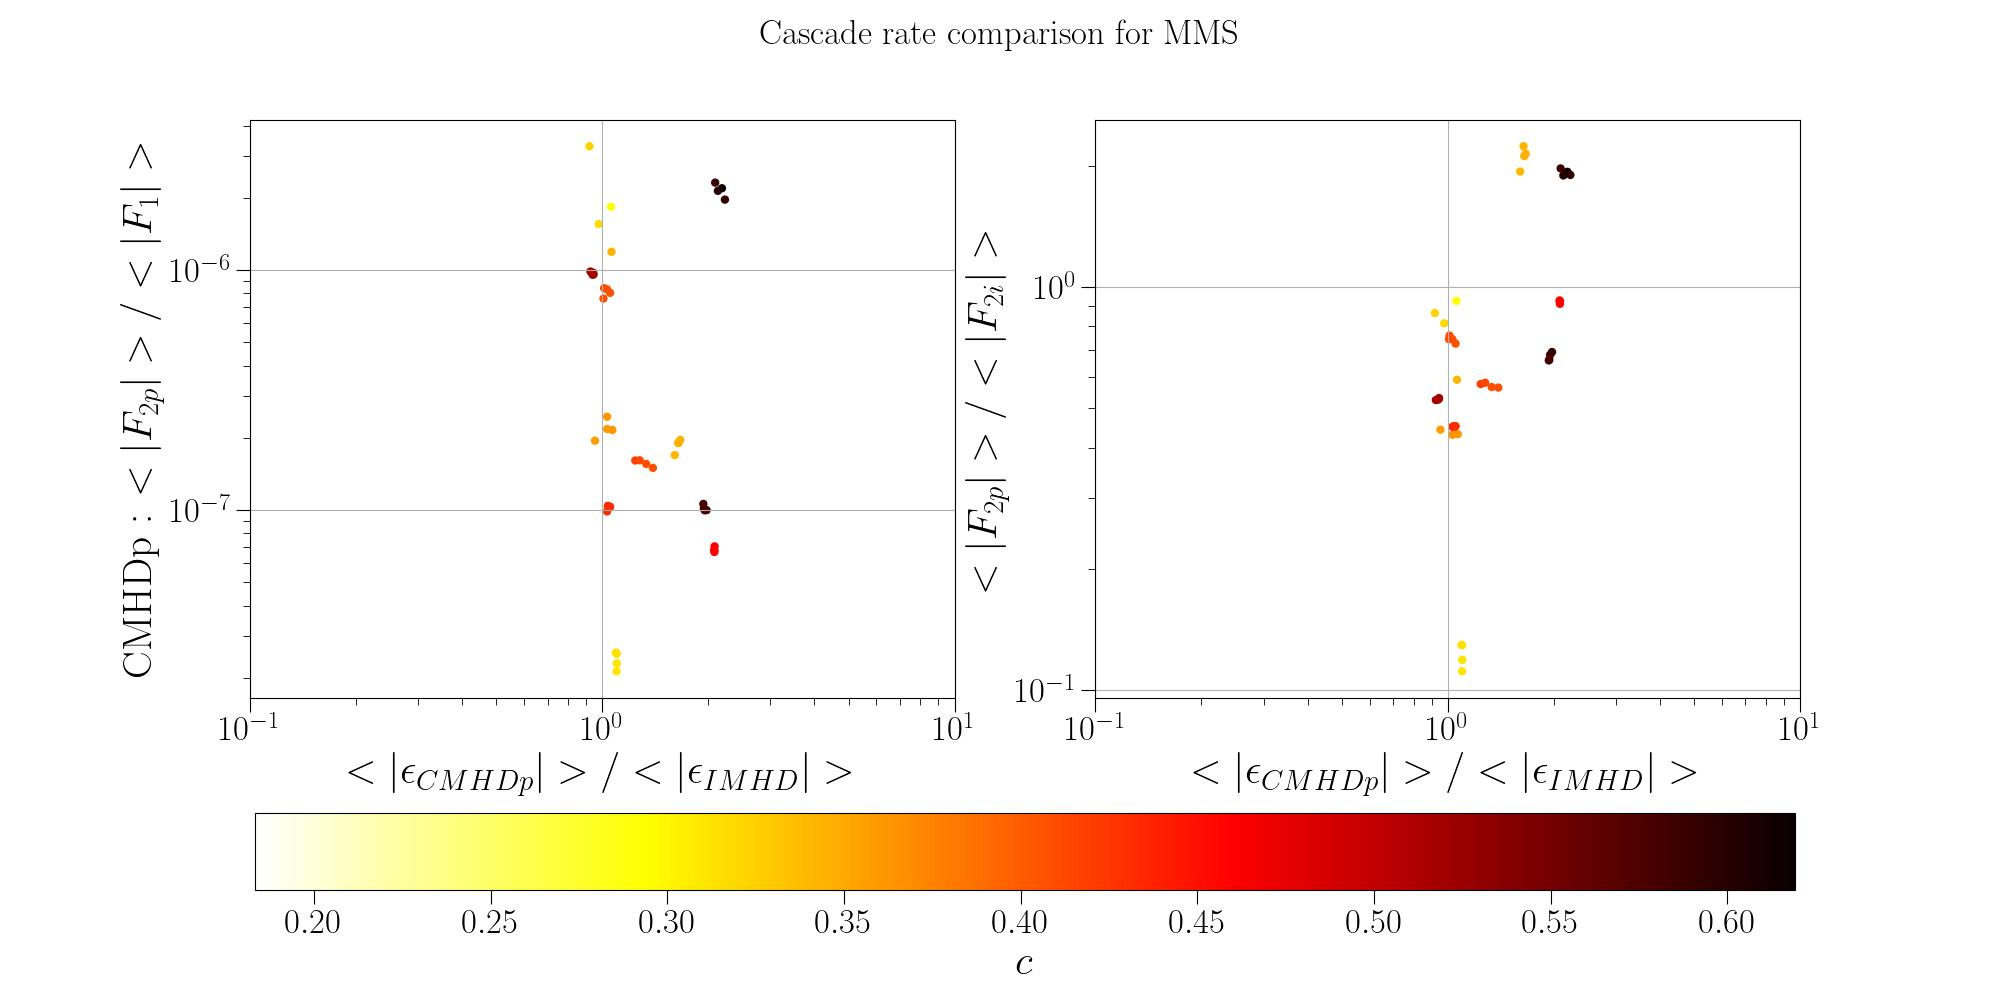
\includegraphics[width=\linewidth,trim=3cm 0cm 3cm 3cm, clip=true]{./Mainmatter/Part_1/images/cascade_comp_MMS_2}
\cprotect\caption{Résumé de l'étude statistique préliminaire menée sur 12 intervalles des quatre satellites de \cacro{MMS}. Couleurs : compressibilité $c $ de l'intervalle. Abscisses : rapport entre le taux de cascade compressible adiabatique (CMHDp, $\gamma = 5/3$) et incompressible (IMHD). À gauche : pour CMHDp, rapport entre les contributions d'énergie interne $F_2$ et Yaglom compressible $F_1$. À droite : rapport entre les contributions d'énergie interne adiabatique $F_{2p}$, et isotherme $F_{2i}$ ($\gamma = 1$).}%
\label{fig:loi_MMS}
\end{figure}

Cette étude révèle de plus importantes fluctuations de densité dans la magnétogaine que celles relevées pour les données de \cacro{PSP}. Dans les cas les plus compressibles, le taux de cascade compressible semble pouvoir doubler par rapport au taux incompressible (points rouges éloignés de la verticale centrale). Cependant, la contribution d'énergie interne moyenne y est encore plus négligeable que dans les données de \cacro{PSP}, 5 à 8 ordres de grandeurs plus faibles que la contribution Yaglom compressible moyenne comme le montre le diagramme de gauche. Sur le diagramme de droite, on voit que $\left<F_{2p}\right>$ à tendance à être un peu plus faible que $\left<F_{2i}\right>$ mais qu'il peut aussi être environ deux fois plus important. Cette dernière observation montre un comportement inverse du comportement moyen observé à tout rayon solaire dans le vent solaire par \cite{brodiano_statistical_2022}, mais demanderait plus de statistique pour être confirmée. 
 
 Cette étude dans les données de \cacro{MMS} est restée préliminaire, l'intérêt du travail ayant dévié vers l'effet de l'anisotropie de pression (voir Partie \ref{part_2}). Par la suite, une autre contribution pourrait être étudiée grâce à la constellation de satellites de \cacro{MMS} : celles des termes sources, impossible à analyser avec \cacro{PSP}. La caractéristique multi-sondes de cette mission peut en effet permettre le calcul complet des lois exactes compressibles. Cela a, par exemple, été effectué dans le cadre isotherme par \cite{andres_energy_2019}. Il serait aussi intéressant d'étudier dans les données les contributions au taux de cascade apportées par les différentes formulations ayant été analytiquement dérivées dans le chapitre précédent, en particulier les contributions des termes flux dépendant des pressions magnétique et thermodynamique, ou celle du flux de chaleur.

\newpage
\section{Synthèse de l'étude de cas observationnels issus des données de PSP}
\label{synt-14}
\fcolorbox{blue}{white}{\begin{minipage}[c]{\linewidth}
\paragraph{Données choisies : } instruments \cacro{SPC}/\cacro{SWEAP} et \cacro{MAGs}/\cacro{FIELDS} présents sur la sonde \cacro{PSP}, mesures relevées le 4 Novembre 2018, comparaison d'un intervalle quasi-incompressible et d'un plus compressible. \\

 \paragraph{Hypothèses nécessaires à l'utilisation de données in-situ issues d'une mission composée d'une seule sonde pour l'estimation de taux de cascade : } 
 \begin{itemize}
     \item taille d'intervalle supérieure à plusieurs fois le temps de corrélation des fluctuations turbulentes,
     \item hypothèse de Taylor, $\boldsymbol{\ell} \sim \boldsymbol{v_0} \tau$,
     \item angle $\theta_{VB}$ quasi-stationnaire,
     \item négligence des termes sources dans la loi exacte, valide si vent subsonique et avec la formulation f1 de la loi exacte \cacro{MHD},
     \item intégration isotrope de la loi exacte, validité à nuancer tant que l'angle $\theta_{VB}$ reste quasi-stationnaire.
 \end{itemize}
\end{minipage}}

 \fcolorbox{red}{white}{\begin{minipage}[c]{\linewidth}
 \paragraph{Loi exacte analysée : } $\varepsilon = F_1 + F_2$ avec
 \begin{eqnarray*}
  F_1 &=& -\frac{3}{4|\boldsymbol{v_0}|\tau}\left<(\delta (\rho\boldsymbol{v}) \cdot \delta \boldsymbol{v}+ \delta (\rho\boldsymbol{v_A}) \cdot \delta \boldsymbol{v_A}) \delta \boldsymbol{v}  -(\delta (\rho\boldsymbol{v_A}) \cdot \delta \boldsymbol{v}  + \delta (\rho\boldsymbol{v}) \cdot \delta \boldsymbol{v_A}  ) \delta \boldsymbol{v_A} \right> \\
  F_2 &=& -\frac{3}{4|\boldsymbol{v_0}|\tau}\left<2 \delta \rho  \delta u  \delta \boldsymbol{v}\right>
 \end{eqnarray*}
 \paragraph{Fermetures : }
 \begin{itemize}
     \item incompressible : $\rho = \rho_0$, pas de $u$ nécessaire,
     \item isentrope-isotherme : $u = c_s^2 \ln(\frac{\rho}{\rho_0})$ et $\gamma = 1$,
     \item isentrope-adiabatique : $u = \frac{c_s^2 -c_{s0}^2}{\gamma(\gamma -1)}$ et $\gamma = 5/3$.
 \end{itemize}
 
 \paragraph{Conclusion : }
 \begin{itemize}
     \item apport potentiellement substantiel de la compression via la densité dans les termes de type $F_1$ indépendant de la fermeture,
     \item apport de la fermeture important dans $F_2$ à petite échelle,
     \item $F_2$ négligeable devant $F_1$ pour les fermetures compressibles et dans les cas analysés.
 \end{itemize}
 
 Ces résultats sont publiés dans \cite{simon_general_2021}, statistiquement validés par \cite{brodiano_statistical_2022} et étendus dans la magnétogaine à travers une étude statistique préliminaire effectuée dans les données de \cacro{MMS} (section \ref{sec-133}). 
 \end{minipage}}
